\section{Background}
% Delete the text and write your Theory/ Background Information here:
%------------------------------------

\subsection{Reinforcment Learning}

Reinforcment learning is defined as the problem that an agent tries to solve by learning behaviour through trial and error with its enviroment. In other words programming an agent through rewards and punishments rather than how to specificaly solve the task itself\cite{kaelbling1996reinforcement} as depicted in figure \ref{figRL}.
\begin{figure}[H]
    \centering
    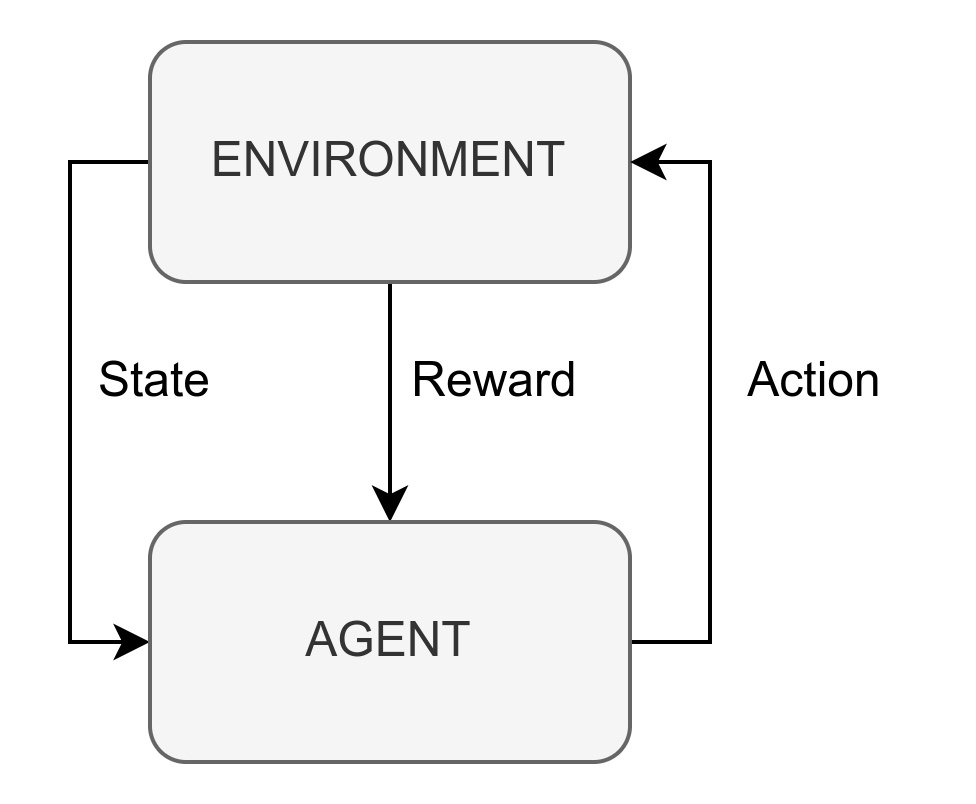
\includegraphics [scale = 0.2]{Images/RL_graph.png}
    \caption{Graph representing reinforcment learning}
    \label{figRL}
\end{figure}
%It can be devided into two strategies for solving said problems. The first strategy involves searching the space or state-action pairs for in order to find which work better in the enviroment. The second technique is estimating the utillity of a particular action. 
The first concept crucial for reinforcment learning is the \textit{reward function} which is objective feedback from the enviroment. It is usually scalar values that are associate with state action pairs. High rewards are usually associate by state-action pairs which benificial for the agent to be situated in whereas negative rewards would then be disadvantageous states or \textit{hazardous} for the agent to be in. Essentially what is good and bad for the agent in the enviroment. The sole objective of the agent is then to maximize this reward\cite{sutton1999reinforcement}.

Naturally we have to define \textit{state} and \textit{action}, which compared to the rest of the concepts have a very general definition. That being the latter is a descision of some sort and the former a factor that has to be taken into considaration when taking an action. 

A central class of methods reinforcment learnign is temporal difference learning. It refers to a class of methods which the learning is based on the difference between temporally successive predictions. It aims to adjust the learner's current expectation for the present input pattern so that it more accurately aligns with the subsequent prediction at the following time step. Unlike Monte carlo methods and other methods in temporal learning updates its estimated value function at every step. \cite{tesauro1995temporal}. 

In temporal learning there are several subcmethods or rather algorithms such as SARSA ,Q learning, TD-Lambda and more \cite{eiben2007reinforcement}. Q learning is an algorithm where the enviroment can be constituted by a controlled Markov process where the agent is controlling it \cite{watkins1992q}. The agent chooses an action and accordingly gets rewarded for it. Q-learning uses the Markov chains to calculate the max reward that can be accumilated by the next state action and updates towards that as shown in the equation below.

\begin{equation} \label{eqQ}
    { Q(s,a) := Q(s,a) + \eta [r + \gamma \max Q(s',a') - Q(s,a)]}
\end{equation}

Equation \ref{eqQ} is the \textit{value} or \textit{update} equation which is responsible for mapping the different states bassed on their estimated long term reward in Q learning. Here $Q(s,a)$ is the current state of the agent $r$ is the reward, $\eta$ is the learning rate and $Q(s',a')$ is the next state. An importnad variable here is $\gamma$ which represent the discount factor. This is used to limit the Markov chain to a limited finite number so they don't end up infinite. This controlls how many steps into the future the agent will try ot estimate. 


\subsection{Genetic Algorithms}

Genteic algorithms are computational models based on the concept of evolution as seen in biology. Similarly to how organisms evolve by natural selection and sexual reproduction, programs can also simulate these processes and behave in a similar fashion to organisms in order to solve a specific problem. In a general sense natural selection is the process which determins which individuals get to survive by some test of fitness. After the best fitted are selelcted the creation or reproduction of the next generation starts. Reproduction is then the method in which the mixing of genes in the remaining population happens and gets passed to the offspring \cite{holland1992genetic}.
\begin{figure}[H]
    \centering
    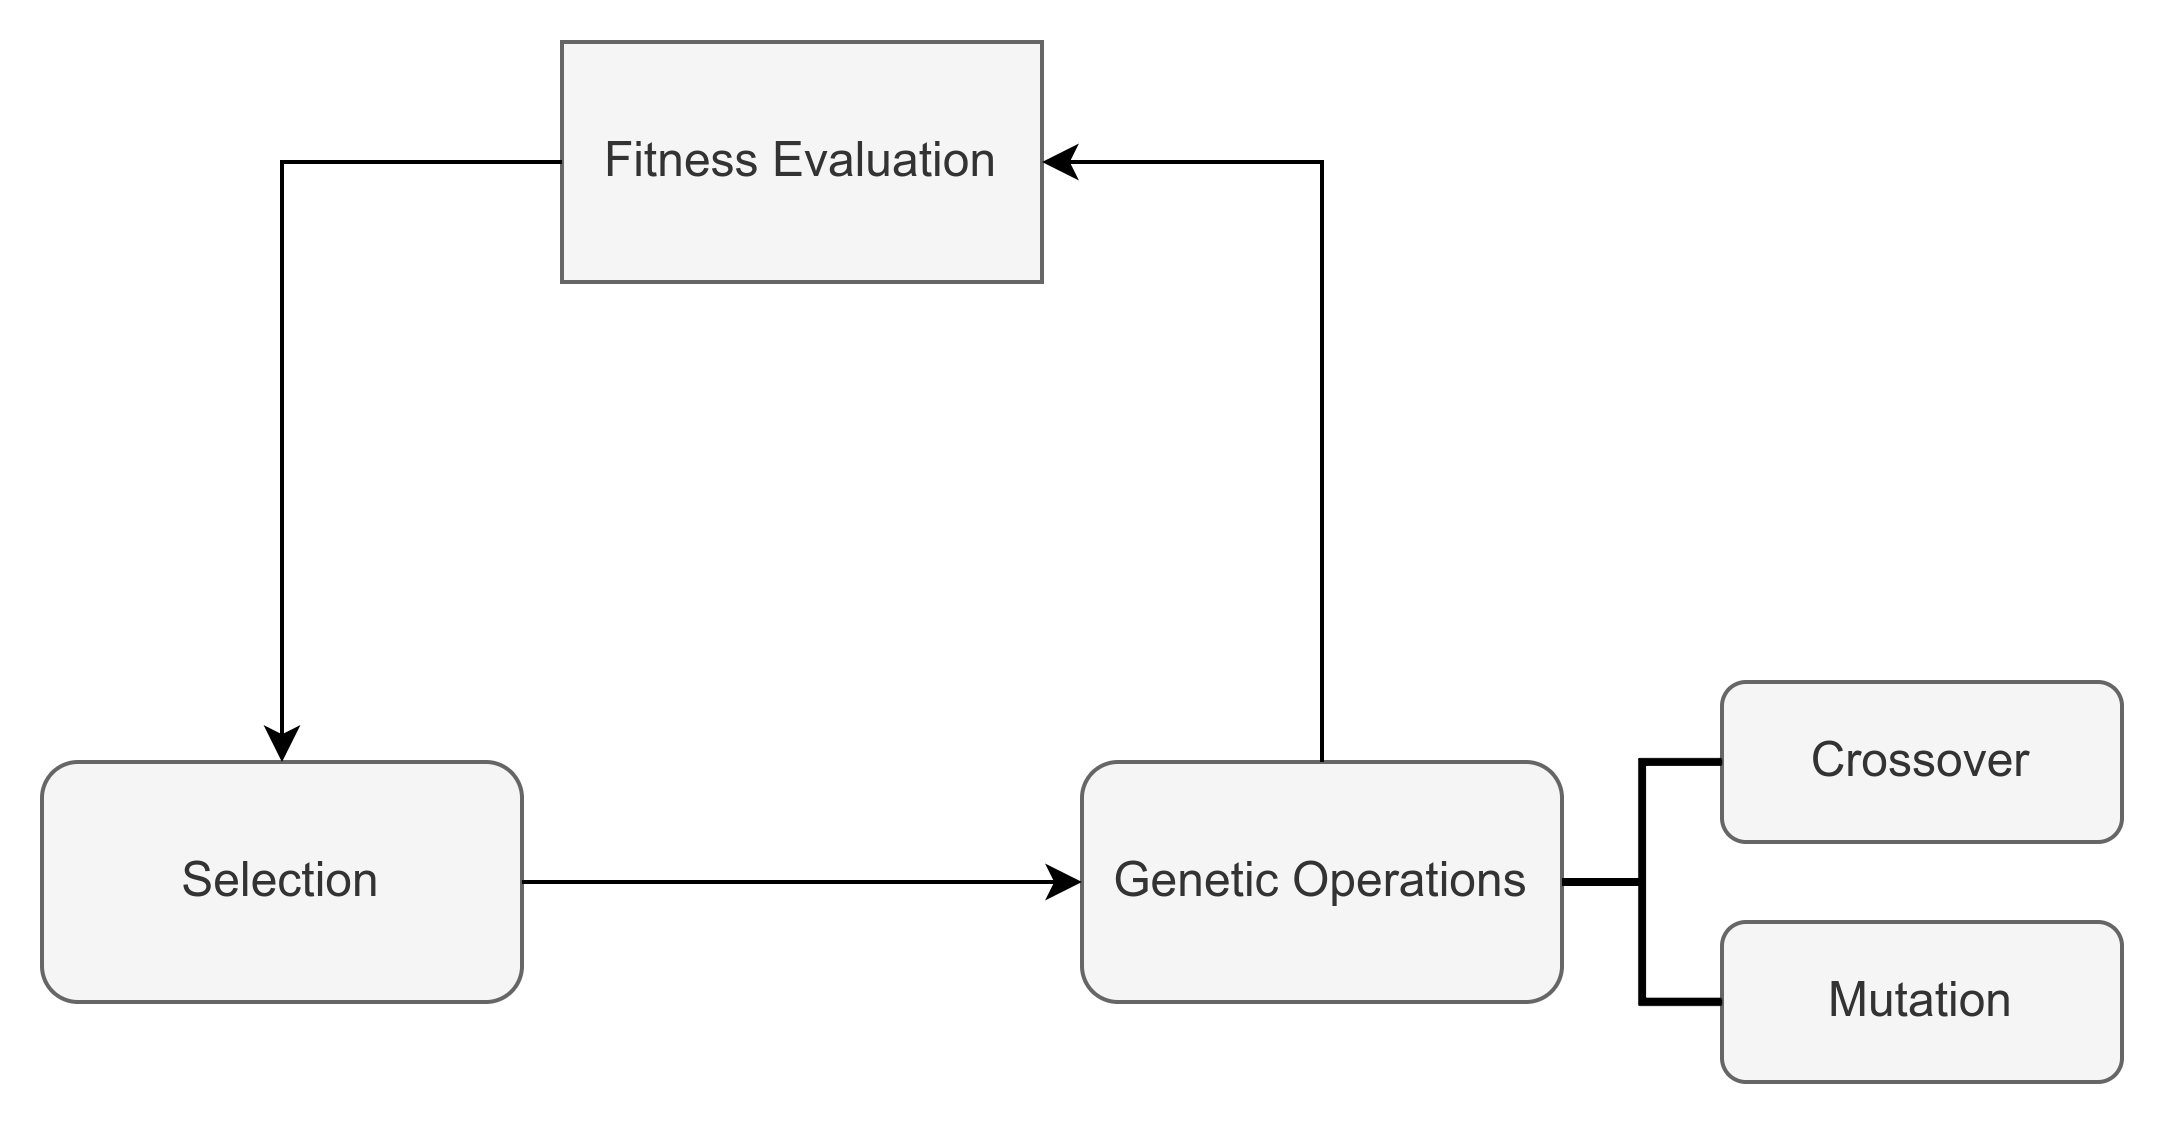
\includegraphics [scale = 0.08]{Images/GA_graph.png}
    \caption{visual representation of genetic algorithms}
    \label{figGA}
\end{figure}

By starting with a population of individuals wich are creaated randomly we have an initial population with variation amongst the individuals. The DNA wich is essentialy the code of the gene can be represented by a string of bits. These string bits can thought as potential solutions to the problem. Due to the variation in the population some individuals vill be better \textit{fit} which then will be selected to remain. In the final stage the remaiining individuals will mix their bit strings to produce individuals for the next generation. These steps will be continually done fore some number of generations \cite{forrest1996genetic}. 

It is importnad however that we reduce the genetic drift and keep track of hte best solutions that have been produced by the previous generation. To do that we employ a method called Elitism. In ellitism compared with traditional reproductiion the most fitting individual are copied to the next generation without any alteration. In that way the best solution of each generation is alway preserved and adds selective preassure and improve convergence speed \cite{du2018elitism}.
% If the theory section is short, you may combine it with the introduction or method section. \par

% This section should provide a short overview of the theoretical background for the experiment. Include all equations (but not elementary/ trivial equations that one can assume the reader knows) that are used in the report. Do not reference the experiment in this section. Rather, write more general and use arbitrary variables in equations (not specific variables for the experiment). \par

% Here are some equations:
% \begin{align} % Use & sign to align, use \nonumber to write a line without number.
%     \laplacian{V} &=0 \nonumber \\
%     \frac{\partial^2 V}{\partial x^2}+\dpd[2]{V}{y} &=0 \label{eq:Laplace} % dpd = display mode partial derivative
% \end{align}

% \Cref{eq:Laplace} % Use \Cref at the start of a sentence and \cref mid sentence.
% is Laplace's equation for electric potentials in two dimensions \parencite[131,136]{Griffiths}. \par
% Here is an example of an equation with different cases:

% \begin{align*} % use equation* or align* to get un-numbered equations.
%     \int_{0}^{a}\sin(nx)\sin(n'x) \dd x = 
%     \begin{cases} 
%         0, \hspace{1cm} \text{if } n'\neq n \\ 
%         \frac{a}{2}, \hspace{1cm} \text{if } n'= n
%     \end{cases}
%     \footnotemark{}
% \end{align*}
% \footnotetext{Notice that the differential operator is \textit{not} italic and that there is a tiny space in front of it.}

% The \verb+NTNU-lab.sty+ includes a some spicy equal signs. For example: 
% \begin{align}
%     \vb{E} & \defeq \frac{\vb{F}}{q} \label{eq:def} \\
%     \vb{E} &\coleq\frac{\vb{F}}{q} \label{eq:col} \\
%     a      &\qmeq b                 \label{eq:qm}  \\
%     G      &\meq \SI{6.6e-11}{m^3 kg^{-1} s^{-2}}  \label{eq:m} 
% \end{align}

% The equality symbols in \cref{eq:def,eq:col} means equal to by definition. Note that these may sometimes be used slightly different from $\triangleq$ (equal to by definition):
% \begin{equation*}
%     a \coleq 3, \hspace{1cm} \Rightarrow \hspace{1cm} a+2 \triangleq 3+2 = 5
% \end{equation*}

% The symbol in \cref{eq:qm} conveys an uncertainty in the statement, as in ``We do not know if $a=b$, but we think it does.'' Such a statement would be followed up by investigating the claim either mathematically or empirically. For example, a paper investigating Ohm's law could state the hypothesis $V\qmeq I\cdot R$ at the start of the paper.\par

% The symbol in \cref{eq:m} is called ``measured by''. Sadly I'm not familiar with how this symbol is used. I can, however, think of two possibilities: \par
% \begin{itemize}
%     \item to define a mathematical object\footnotemark{} by measurement(s) (similar to $\defeq$)
%     \item to specify the measured value of a mathematical object.
% \end{itemize}

% \footnotetext{I used this word as an umbrella term for variables, constants, vectors, tensors and other things that can be measured/ found empirically.}

% \begin{figure}
% \centering
% \begin{circuitikz} \draw
%     (0,0) to[V=15<\volt>] (0,6) to [short, -*, i=50<\milli \ampere>]
%     (2,6) to[R, l=$R_1$] (2,4) 
%     to[R, l=$R_2$] (2,2)
%     to[R, l=${R_3=R_2}$] (2,0) -- (0,0)
%     (2,6) to[short, -*] (4,6)
%     (2,0) -- (4,0)
%     (4,0) to[short, -o] 
%     (4,2)
%     (4.5,1.3) node[label={b}] {}
%     (4,6) to[short,i=$I$,-o] 
%     (4,4)
%     (4.5,4) node[label={a}] {}
%     ;
%     \node[draw,minimum width=1.3cm,minimum height=2cm] at (4,3){Load};
%     \draw [decorate,decoration={brace,amplitude=6pt,mirror,raise=4pt},yshift=0pt]
%     (4.7,2) -- (4.7,4) node [black,midway,xshift=0.8cm] {\footnotesize
%     $R_{\textnormal{Load}}$};
%     \draw[red, thick] (1.5,5.5) rectangle (4.5,6.5)
%     node[pos=0.5, above]{KCL};
%     %\node[] at (2,7){}; % This empty node is used to get some space between the text.

% \end{circuitikz}
% \caption{A circuit diagram. We can apply Kirchhoff's current law (KCL) in the red box and Ohm's law to figure out the unknown values.}
% \label{fig:Circuit}
% \end{figure}

% An example of the first usage would be the gravitational constant, which numerical definition relies on measurements: $G \meq \SI{6.67430(15)e-11}{m^3 kg^{-1} s^{-2}}$.\cite{G_constant} \par
% To give an example of the second way to use the symbol, let us assume you measured a current $I_1$ to be $\SI{3.3(1)}{A}$. Then, you would simply write $I_1\meq \SI{3.3(1)}{A}$, and it would imply that this value was measured (without the need to explicitly mention this in the text). \par
% Personally, I would chose the latter way of using the symbol, simply because this way of using it would occur more frequently in undergraduate reports than the former.
% If you chose to use this symbol, I would recommend clarifying how you use it in a footnote. That is, if its meaning is unclear and/or ambiguous given the context. \par


% \Cref{fig:Circuit} shows a circuit diagram drawn using \verb+circuitikz+. \Cref{tab:Circuit_table} shows possible values for the circuit and is an example of a table with a coloured row. It also shows an example of using footnotes inside tables (normal footnotes inside tables will not be displayed).

% \begin{table}[htb]
%     \centering
%     \begin{tabular}{|c|c|c|}
%          \hline
%          \rowcolor{pink}
%         $R_{\textnormal{Load}}$ & $I$ & $R_1+R_2+R_3$\tablefootnote{This is the same as $2 R_1+R_2$} \\
%         \rowcolor{pink}
%         $(\si{\ohm})$ & $(\si{\milli \ampere})$ & $(\si{\ohm})$ \\
%          \hline
%         350 & 42.9 & 2100 \\
%         400 & 37.5 & 1200 \\
%         500 & 30 & 750 \\
%         1000 & 15 & 428.6 \\
%         1300 & 11.5 & 390 \\
%          \hline
%     \end{tabular}
%     \caption{Some values for the circuit in fig. \ref{fig:Circuit}.}
%     \label{tab:Circuit_table}
% \end{table}